\documentclass{beamer}

\usepackage{amsmath}
\usepackage{stmaryrd}
\usepackage{xspace}


\usepackage{comment}
\usepackage{multirow}
\usepackage{tikz}

\input{macros.tex}

%%%%%%%%%%%%%%%%%%% Title Page Info%%%%%%%%%%%%%%%%%%%%%%%%%%

\title{Characteristic Bisimulations for Higher-Order Session Types}

\author{{\bf Dimitrios Kouzapas$^{1,3}$}, Jorge A. P\'{e}rez$^{2}$, and Nobuko Yoshida$^1$}

\institute{Imperial College London$^1$, University of Groningen$^2$, University of Glasgow$^3$}

\date

\begin{document}
	\begin{frame}
		\titlepage
	\end{frame}

	\begin{frame}{Higher-Order Calculi}
		\begin{itemize}
			\item	Higher-order calculi may communicate processes as values.
		\end{itemize}

		\[
			\bout{n}{\abs{y}{R}} P \Par \binp{\dual{n}}{x} Q \red P \Par Q \subst{\abs{y}{R}}{x}
		\]
	\end{frame}

	\begin{frame}{Higher-Order Sessions}
		\begin{itemize}
			\item	\HOp is a higher-order calculus that specifies session protocols
		\end{itemize}

		\[
			\tree {
				\Gamma; \Lambda_1; \Delta_1 \cat n: S_2 \proves P \hastype \Proc
				\qquad
				\Gamma; \Lambda_2; \Delta_2 \cat x: S_1 \proves \abs{x}{Q} \hastype \shot{S_1}
			}{
				\Gamma; \Lambda_1 \cat \Lambda_2; \Delta_1 \cat \Delta_2 \cat n: \btout{\shot{S_1}} S_2 \proves \bout{n}{\abs{x}{Q}} P \hastype \Proc
			}
		\]
	\end{frame}

	\begin{frame}{Bisimulation for Higher-Order Sessions}
		\begin{itemize}
			\item	Contextual Bisimulation is a well known behavioural equivalence for Higher-Order calculi.
			\item	Contextual Bisimulation is based on heavy quantifications on output and input clauses.
			\item	Sangiorgi and, subsequently Jeffrey and Rathke offered alernative behavioural characterisations
				in the untyped setting that do not suffer from universal quantification clauses.
		\end{itemize}
	\end{frame}

	\begin{frame}{Bisimulation for Higher-Order Sessions}
		\begin{itemize}
			\item	We work on the typed setting using as a basis \HOp.
			\item	The linear nature of session types allows to define yet
				another behavioural characterisation for typed Higher-order calculi
				which we call {\em Characteristic Bisimulation}.
			\item	The bisimulation is defined on a refined labelled transition system
				that restricts process actions following the session behaviour.
			\item	A further interesting result is that, due to types, the proofs do
				not require the presence of a name matching construct.
		\end{itemize}
	\end{frame}

	\begin{frame}{Higher-Order Contextual Bisimulation: Output}
		Suppose $P \,\Re\, Q$, for some context bisimulation~$\Re$. Then:
		\begin{enumerate}[$(\star)$]
			\item	Whenever
				\[
					P \by{\news{\widetilde{m_1}} \bactout{n}{V}} P'
				\]
				there exist $Q'$ and $W$ such that 
				\[
					Q \By{\news{\widetilde{m_2}} \bactout{n}{W}} Q'
				\]
				and, \fbox{\emph{\textbf{for all} $R$}}  with $\fv{R}=x$, 
				\[
					\newsp{\widetilde{m_1}}{P' \Par R\subst{V}{x}}\ \Re\ \newsp{\widetilde{m_2}}{Q' \Par R\subst{W}{x}}
				\]
		\end{enumerate}
	\end{frame}

	\begin{frame}{Higher-Order Contextual Bisimulation: Output}
		Equivalently rewrite the conclusion of the ($\star$) clause:
		\\[2mm]

		Suppose $P \,\Re\, Q$, for some context bisimulation~$\Re$. Then:
		\begin{enumerate}[$(\star)$]
			\item	Whenever\\
				\dots\\
%				\[
%					P \by{\news{\widetilde{m_1}} \bactout{n}{V}} P'
%				\]
%				there exist $Q'$ and $W$ such that 
%				\[
%					Q \By{\news{\widetilde{m_2}} \bactout{n}{W}} Q'
%				\]
%				and,
				\dots \emph{\textbf{for all} $R$}  with $\fv{R}=x$, 
				\[
					\begin{array}{c}
						\newsp{\widetilde{m_1}}{P' \Par \newsp{s}{\binp{s}{x} R \Par  \bout{s}{V} \inact}}
						\\
						\Re
						\\
						\newsp{\widetilde{m_2}}{Q' \Par \newsp{s}{\binp{s}{x} R \Par \bout{s}{W} \inact}}
					\end{array}
				\]
				This is because:
				\[
					\begin{array}{c}
						\newsp{s}{\binp{s}{x} R \Par \bout{s}{V} \inact}
						\by{\tau}
						R \subst{V}{x}
						\\
						\newsp{s}{\binp{s}{x} R \Par \bout{s}{W} \inact}
						\by{\tau}
						R \subst{W}{x}
					\end{array}
				\]
		\end{enumerate}
	\end{frame}

	\begin{frame}{Higher-Order Contextual Bisimulation: Output}
		We can further the $(\star)$ clause as a \underline{non universally quantified} input triggered context:
		\\[2mm]

		Suppose $P \,\Re\, Q$, for some context bisimulation~$\Re$. Then:
		\begin{enumerate}[$(\star)$]
			\item	Whenever\\
				\dots\\
%				\[
%					P \by{\news{\widetilde{m_1}} \bactout{n}{V}} P'
%				\]
%				there exist $Q'$ and $W$ such that 
%				\[
%					Q \By{\news{\widetilde{m_2}} \bactout{n}{W}} Q'
%				\]
%				and,
				%\dots \emph{\textbf{for all} $R$} with $\fv{R}=x$, 
				\[
					\begin{array}{c}
						\newsp{\widetilde{m_1}}{P' \Par \binp{t}{y}\newsp{s}{\binp{s}{z} \appl{y}{z} \Par \bout{s}{V} \inact}}
						\\
						\Re
						\\
						\newsp{\widetilde{m_2}}{Q' \Par \binp{t}{y}\newsp{s}{\binp{s}{z} \appl{y}{z} \Par \bout{s}{W} \inact}}
					\end{array}
				\]
		\end{enumerate}

		This is because:

		\emph{\textbf{for all} $R$} with $\fv{R}=x$, 
		\[
			\begin{array}{c}
			\binp{t}{y}\newsp{s}{\binp{s}{z} \appl{y}{z} \Par \bout{s}{V} \inact}
			\by{\bactinp{t}{\abs{x}{R}}} \by{\tau}
			R \subst{V}{x}
			\\
			\binp{t}{y}\newsp{s}{\binp{s}{z} \appl{y}{z} \Par \bout{s}{W} \inact}
			\by{\bactinp{t}{\abs{x}{R}}} \by{\tau}
			R \subst{W}{x}
			\end{array}
		\]
	\end{frame}

	\begin{frame}{Higher-Order Contextual Bisimulation: Input}
		Suppose $P \,\Re\, Q$, for some context bisimulation~$\Re$. Then:
		\begin{enumerate}[$(\bullet)$]
			\item	\fbox{\emph{\textbf{For all} $V$}} such that:
				\[
					P \by{\bactinp{n}{V}} P'
				\]
				then there exists $Q'$ such that
				\[
					Q \By{\bactinp{b}{V}} Q'
				\]
				and
				\[
					P'\ \Re\ Q'
				\]
		\end{enumerate}
	\end{frame}

	\begin{frame}{Higher-Order Contextual Bisimulation: Input}
		We can take advantage of session types to improve the
		$(\bullet)$ clause.
		\vspace{3mm}

		\begin{definition}[Characteristic Process]
			A session type $S$ can be inhabited by a simple
			{\em characteristic} process, $\omapchar{S}$.
%			where $u$ is a name.
		\end{definition}
		\vspace{3mm}

		For example session:
		\[
			S = \btinp{\shot{S_1}} \btout{S_2} \tinact
		\]
		is inhabited by {\em characteristic process}:
		\[
			\omapchar{S} = \binp{u}{x} (\bout{u}{s_2} \inact \Par \appl{x}{s_1})
		\]
		for a fresh name $u$.
	\end{frame}

	\begin{frame}{Higher-Order Contextual Bisimulation: Input}
		We can now define a refined bisimulation relation
		using a new reduction relation, where the input action
		clause maintains the property:
		\\[4mm]

		Suppose $P \,\Re\, Q$, for some {\em characteristic} bisimulation~$\Re$. Then:
		\begin{enumerate}[$(\bullet)$]
			\item	Whenever {\em we expect to input a value of type $U$} on P:
				\[
					P \hby{\bactinp{n}{\omapchar{U}}} P'
				\]
				then there exists $Q'$ such that
				\[
					Q \Hby{\bactinp{n}{\omapchar{U}}} Q'
				\]
				and
				\[
					P'\ \Re\ Q'
				\]
		\end{enumerate}
	\end{frame}

	\begin{frame}{Contextual Bisimulation for Higher-Order Sessions}
		
	\end{frame}
	


\begin{comment}
\begin{definition}[Characteristic Bisimilarity]\rm
	\label{d:fwb}
A typed relation $\Re$ is a {\em  characteristic bisimulation} if 
for all $\horel{\Gamma}{\Delta_1}{P_1}{\ \Re \ }{\Delta_2}{Q_1}$, 
\begin{enumerate}[1)]
\item 
	Whenever 
	$\horel{\Gamma}{\Delta_1}{P_1}{\hby{\news{\widetilde{m_1}} \bactout{n}{\dk{V_1: U}}}}{\Delta_1'}{P_2}$ %with $\Gamma; \es; \Delta \proves V_1 \hastype U$,  
	then there exist 
	$Q_2$, $V_2$, $\Delta'_2$ such that 
	$\horel{\Gamma}{\Delta_2}{Q_1}{\Hby{\news{\widetilde{m_2}}\bactout{n}{\dk{V_2: U}}}}{\Delta_2'}{Q_2}$ %with $\Gamma; \es; \Delta' \proves V_2 \hastype U$,  
	and, for fresh $t$, \\ 
	$%\begin{array}{lrlll}
	\Gamma; \Delta''_1  \proves  {\newsp{\widetilde{m_1}}{P_2 \Par 
	\ftrigger{t}{V_1}{U_1}}}
	  \,\Re\,
	 \Delta''_2 \proves {\newsp{\widetilde{m_2}}{Q_2 \Par \ftrigger{t}{V_2}{U_2}}}
%\end{array}
$
		
\item	
For all $\horel{\Gamma}{\Delta_1}{P_1}{\hby{\ell}}{\Delta_1'}{P_2}$ such that 
$\ell$ is not an output, 
 there exist $Q_2$, $\Delta'_2$ such that 
$\horel{\Gamma}{\Delta_2}{Q_1}{\Hby{\hat{\ell}}}{\Delta_2'}{Q_2}$
			and
			$\horel{\Gamma}{\Delta_1'}{P_2}{\ \Re \ }{\Delta_2'}{Q_2}$; and 

                      \item	The symmetric cases of 1 and 2.                
	\end{enumerate}
	The largest such bisimulation
	is called \emph{characteristic bisimilarity} \jpc{and} denoted by $\fwb$.
\end{definition}
\end{comment}

\end{document}


\begin{comment}
\newcommand{\Doctor}{\textsf{Doctor}}
\newcommand{\DBAdmin}{\textsf{DBAdmin}}
\newcommand{\Nurse}{\textsf{Nurse}}
\newcommand{\Hospital}{\textsf{Hospital}}
\newcommand{\Hosp}{\textsf{Hosp}}

\newcommand{\newG}[2]{(\nu\ #1)(#2)}
\newcommand{\group}[2]{#1[#2]}
\newcommand{\iotypes}{\mathtt{i/o}}

\newcommand{\rtype}{\mathtt{r}}
\newcommand{\wtype}{\mathtt{w}}
\newcommand{\etype}{\mathtt{e}}
\newcommand{\rwtype}{\mathtt{rw}}

\newcommand{\psend}[2]{\send{#1}\freev{#2}.}
\newcommand{\precv}[2]{\receive{#1}\boundv{#2}.}

\newcommand{\Serverone}{\textsf{Server}_1}
\newcommand{\Servertwo}{\textsf{Server}_2}
\newcommand{\Client}{\textsf{Client}}

\newcommand{\sone}{\mathtt{r}_1}
\newcommand{\stwo}{\mathtt{r}_2}
\newcommand{\crole}{\mathtt{c}}

\newcommand{\tikzsize}{\tiny}

\newcommand{\instrument}{\mathtt{i}}
\newcommand{\agentone}{\mathtt{a}_1}
\newcommand{\agenttwo}{\mathtt{a}_2}
\newcommand{\user}{\mathtt{u}}

\begin{document}

\title{A Typing System for Privacy}
\author{Dimitrios Kouzapas$^{1}$ and Anna Philippou$^2$}
\institute{
	Department of Computing Science, University of Glasgow\inst{1}\\
	Department of Computer Science, University of Cyprus\inst{2}
}
\date{}

\begin{frame}
	\titlepage
\end{frame}

\begin{frame}{What is Privacy?}
%
	\begin{itemize}
		\item	Privacy as a general concept does not have a single definition.
		\item	Various definitions for privacy are subject to philosophy, 
			legal systems and societies in general.
		\item	From a legal point of view privacy can be seen as a collection
			of individual's rights.
	\end{itemize}
%
\end{frame}

\begin{frame}{Why Privacy?}
%
	\begin{itemize}
		\item	Privacy in information technology presents a huge challenge.

		\item	Clouds and Databases allow the aggregation of sensitive 
			information over individuals.

		\item	Networks and network applications such as e-commerce or
			social networks allow for public sharing of private data.

%		\item	Information technology may change today's notion of
%			privacy.
		\item	Technology creates new challenges for the privacy of data.

		\item	Technology can help in preserving the privacy of data.

		\item	People that handle sensitive information need to
			protect the data subjects and protect themselves
			against the law.		
	\end{itemize}
%
\end{frame}

\begin{frame}{Privacy and Formal Methods}
%
	\begin{itemize}
		\item	\textrm{M. C. Tschantz and J. M. Wing. 
				Formal methods for privacy.
				In Proceedings of FM, LNCS 5850, Springer, 2009.}
		\item	A study that discusses the need for formal methods
			for understanding and preserving privacy as information
			technology advances.

		\item	The arguments follow a taxonomy on privacy violation from Solove:
			\begin{itemize}
				\item	Invasion.
				\item	\alert<2>{Information collection}
				\item	\alert<2>{Information processing}
				\item	\alert<2>{Information dissemination}
			\end{itemize}
	\end{itemize}
%
\end{frame}

\begin{frame}{Privacy}
%
		\begin{itemize}
			\item	{\bf Privacy:}	A \alert<1,2>{data holder} is responsible to protect 
						private information about a \alert<1,2>{data subject}
						against unauthorised (and authorised) \alert<1,2>{adversaries}.
			\pause
			\item	{\bf Security:}	An entity in a system is responsible for
						preserving the security properties of the system.
		\end{itemize}
%
\end{frame}

\begin{frame}{Privacy and Behavioural Types}
%
	\begin{itemize}
		\item	The $\pi$-calculus.
		\item	Rich theory in operational, behavioural and typing semantics.
		\item	Use the $\pi$-calculus meta-theory (and other machinery) to abstract the privacy model
			and concepts.
			%using the $\pi$-calculus meta-theory machinery to model privacy concepts.
	\end{itemize}
%
\end{frame}

\begin{frame}{\only<1>{Presentation Through Example}\only<2,3,4,5>{Information }\only<2,3>{Collection}\only<4>{Processing}\only<5>{Dissemination}}
	\only<1>{
		A \textbf{Data Base Administrator} (\alert<1>{data holder}) 
		sends \textbf{Patient's} (\alert<1>{data subject}) data
		to a \textbf{Doctor} (\alert<1>{authorised adversary}), using
		a \textbf{Nurse} (\alert<1>{unauthorised adversary}) as a delegate.
	}
	\only<2,3>{
		Use of the $\pi$-calculus with groups to
		prevent eavesdropping from external
		unauthorised adversaries.
		\vspace{16pt}
	}
	\only<4>{
		Use of the $\iotypes$ types for the $\pi$-calculus
		to prevent access from unauthorised adversaries.
		\vspace{16pt}
	}
	\only<5>{
		Use of the notion of linear usage of names to control 
		information dissemination to unauthorised adversaries.
		\vspace{16pt}
	}
%
	\begin{center}
		\begin{tikzpicture}
	%		\draw[dashed]	(0,0) -- (9, 0) (0,0)--(0,3) ;

			\draw[rounded corners]	(0, 2) rectangle (1.5, 1)
						(3.75, 2) rectangle (5.25, 1)
						(7.50, 2) rectangle (9, 1);

			\node at		(0.75, 1.5) {\footnotesize \textsf{DB Admin}};
			\node at		(4.5, 1.5) {\footnotesize \alert<4>{\textsf{Nurse}}};
			\node at		(8.25, 1.5) {\footnotesize \textsf{Doctor}};

			\draw[->, very thick]	(1.5, 1.5) -- (3.75, 1.5);
			\draw[->, very thick]	(5.25, 1.5) -- (7.50, 1.5);

			\node at		(2.625 ,1.8) {\footnotesize \textsf{Patient's Data}};
			\node at		(6.375 ,1.8) {\footnotesize \textsf{Patient's Data}};

			\only<2,3,4,5>{
			\draw[dashed]		(4.5, 1.5) ellipse (5 and 1.5);
			\node at		(3.75, 0.5) {\alert<2,3>{\Hospital}};
			}
			\only<1>{
			\draw[very thin, gray, dash pattern = on 1pt off 75pt]	(4.5, 1.5) ellipse (5 and 1.5);
			}

			\only<4,5>{
			\node at		(0.75, 2.2) {\alert<4>{$\rwtype$}\only<5>{\alert<5>{*}}};
			\node at		(4.5, 2.2) {\alert<4>{$\etype$}\only<5>{\alert<5>{1}}};
			\node at		(8.25, 2.2) {\alert<4>{$\rwtype$}\only<5>{\alert<5>{0}}};
			}
		\end{tikzpicture}
	\end{center}
%
	\[
		\visible<2,3,4,5>{(\nu\ \Hospital)(}\DBAdmin \Par \Nurse \Par \Doctor\visible<2,3,4,5>{)} \visible<3>{\alert<3>{\Par External}}
	\]

\end{frame}

\begin{frame}{Putting it All Together}
%
\[
	\begin{array}{rcl}
		\DBAdmin &=& \alert<3>{\psend{a}{\alert<2>{c}}} \inact\\
		\Nurse &=& \alert<3>{\precv{a}{x}} \alert<4>{\psend{b}{x}} \inact\\
		\Doctor &=& \alert<4>{\precv{b}{z}} \precv{z}{y} \psend{z}{\mathsf{data}} \inact
	\end{array}
\]
%
	\only<1,2>{
	\visible<2>{Channel \alert<2>{$c$} is used to access the data of the Patient (\alert<2>{data subject}).}
	\vspace{16mm}
	}

	\only<3,4,5>{Channel Types (We omit the group types):}
	\only<6>{ Solution (We omit the group types):}

$ $\\

	\only<3,4,5,6>{
		\begin{tabular}{rcll}
			Channel $a$	& &	\only<3,4,5>{$c: [T]^{\etype1}$ & $a: [[T]^{\etype1}]^{\rwtype0}$\\}
						\only<6>{$c: [T]^{\etype1}, [T]^{\rwtype1}$ & $a: [T_c, T_c']^{\rwtype0}, [T_c, T_c']^{\rwtype0}$\\}
					& &	\only<3,4,5>{\alert<5>{$x: [T]^{\etype1}$}\\}
						\only<6>{\alert<6>{$x: [T]^{\etype1}, [T]^{\rwtype1}$}\\}
			\visible<4,5,6>{
			Channel $b$	& &	\only<3,4,5>{\alert<5>{$z: [T]^{\rwtype0}$} & $b: [[T]^{\rwtype1}]^{\rwtype0}$\\}
						\only<6>{\alert<6>{$z: [T]^{\rwtype0}, [T]^{\rwtype1}$} & $b: [T_c', T_c']^{\rwtype0}, [T_c', T_c']^{\rwtype0}$\\}
			}
		\end{tabular}
	}

	\visible<5>{
		Cannot use sub-typing to go from type $x: [T]^{\etype1}$ to type $z: [T]^{\rwtype0}$.
	}
	\visible<6>{
		Devise a type structure that allows us to control access (using a typing system).
	}
\end{frame}

\begin{frame}{The Typing System}
	\begin{itemize}
		\item Types:
\[
			\begin{array}{rcll}
				\mathsf{T} & \bnfis & G[]^{p\lambda} \bnfbar G[T]^{p\lambda}\\
				p & \bnfis & \etype \bnfbar \rtype \bnfbar \wtype \bnfbar \rwtype\\
				\lambda & \bnfis & * \bnfbar i & i \geq 0
			\end{array}
\]

		\item Subtyping: 
			\begin{itemize}
				\item input co-variance and output contra-variance 
				\item co-inductive definition
				\item based on the pre-orders:
				\[ 
					\begin{array}{c}
						\rwtype \sqsubset_p \rtype \qquad \rwtype_p \sqsubset_p \wtype \qquad \rtype \sqsubset_p \etype 
						\qquad \wtype \sqsubset_p \etype\\
						* \sqsubset_{\lambda} i \qquad i \sqsubset_{\lambda} j\ \ \textrm{ if } i > j
					\end{array}
				\]
			\end{itemize}
		\item Type Structure: ($T_1, T_2$), related by sub-typing.
		\end{itemize}
\end{frame}

\begin{frame}{The Typing System}
	\only<1>{Subsumption:
			\[
			\begin{array}{c}
				\tree{
					\Pi, \Ga\cat x: (T_1', T_2') \proves P \qquad T_1' \leq T_1 \qquad T_2' \leq T_2
				}{
					\Pi, \Ga\cat x: (T_1, T_2) \proves P
				}\\
				\\
				\\
				\tree{
					\Ga \proves x \hastype (T_1', T_2')  \qquad T_1' \leq T_1 \qquad T_2' \leq T_2
				}{
					\Ga \proves x \hastype (T_1, T_2)
				}
			\end{array}
			\]
		}
	\only<2>{Input:
			\[
				\tree{
					\Pi, \Ga\cat y:(T_1, T_2) \proves P \qquad \Ga \proves x \hastype (G[T_1]^{\rtype0}, G[T_2]^{\rtype0})
				}{
					\Pi, \Ga \proves \precv{x}{y} P
				}
			\]
		}
	\only<3>{Output:
			\[
				\tree{
					\Pi, \Ga\cat y:(G_y[T_1]^{\etype\lambda}, T_2) \proves P \qquad 
					\Ga \proves x \hastype (G_x[T_2]^{\wtype0}, G_x[T_2]^{\wtype0})
				}{
					\Pi, \Ga\cat y:(G_y[T_1]^{\etype\lambda\oplus 1}, T_2) \proves \psend{x}{y} P
				}
			\]
		}
\end{frame}

\begin{frame}{Subject Reduction}
	We use auxiliary Lemmas:
	\begin{itemize}
		\item	Weakening
		\item	Strengthening
		\item	Substitution
		\item	Subject Congruence
	\end{itemize}

$ $\\
$ $\\

	\begin{tabular}{rl}
		Theorem: \\
			& If $\Pi, \Ga \proves P$ and $P \red^* P'$ then $\Pi, \Ga \proves P'$.
	\end{tabular}
\end{frame}

\begin{frame}{Complete Hospital Example}
\[
	\begin{array}{rcl}
		\DBAdmin & = & \news{b:T_b} \psend{\mathsf{tonurse}}{b} \psend{\mathsf{todoc}}{b} \psend{a}{c} \inact\\
		\Nurse & = & \precv{\mathsf{tonurse}}{z} \precv{a}{x} \psend{z}{x} \inact\\
		\Doctor & = & \precv{\mathsf{todoc}}{z} \precv{z}{x} \precv{x}{y} \psend{x}{\mathsf{\mathsf{data}}} \inact
	\end{array}
\]

The processes are composed together inside the hospital ($\Hosp$) group.
\[
	\Hospital = \newsp{\Hosp}{\newsp{c : Tc}{\DBAdmin} \Par \Nurse \Par \Doctor}
\]
\end{frame}

\begin{frame}{Complete Hospital Example - Types}
\[
	\Hospital = \newsp{\Hosp}{\newsp{c : Tc}{\DBAdmin} \Par \Nurse \Par \Doctor}
\]
\[
\scriptsize
\begin{array}{rclrcl}
	T_{\mathsf{data}} & = & \Hosp[]^{\etype*} & T_c &=& \Hosp[T_{\mathsf{data}}]^{\rwtype*}\\
	T_a & = & \Hosp[\Hosp[T_{\mathsf{data}}]^{\etype1}]^{\rwtype0} & T_a' &=& \Hosp[T_c]^{\rwtype0}\\
	T_b & = & \Hosp[\Hosp[T_{\mathsf{data}}]^{\rwtype0}]^{\rwtype2}\\
	T_b^n & = & \Hosp[\Hosp[T_{\mathsf{data}}]^{\rwtype0}]^{\wtype0}\\
	T_b^d & = & \Hosp[\Hosp[T_{\mathsf{data}}]^{\rwtype0}]^{\rtype0}\\
	T_{td} & = & \Hosp[T_b^n]^{rw0} & T_{tn} & = & \Hosp[T_b^d]^{rw0}
\end{array}
\]
\[
\scriptsize
\begin{array}{rclrclrcl}
	D &=& (T_{\mathsf{data}}, T_{\mathsf{data}}) & C & = & (T_c, T_c) & A & = & (T_a, T_a')\\
	B &=& (T_b, T_b) & TD & = & (T_{td}, T_{td}) & TN & = & (T_{tn}, T_{tn})
\end{array}
\]
We can show that:
\[
	b: B \cat c: C, \mathsf{tonurse}: TN \cat \mathsf{todoc}: TD \cat a:A \cat \mathsf{data}: D \proves \Hospital
\]

\end{frame}


\begin{frame}{Future Directions}
	\begin{itemize}
		\item	Examples that handle Systems:
			\begin{itemize}
				\item	Search Engines
				\item	Clouds
				\item	Social Networks
				\item	E-commerce
			\end{itemize}

		\item	Examples that handle more issues on privacy:
			\begin{itemize}
				\item	Eavesdropping
				\item	Aggregation - Identification
				\item	Disclosure
				\item	etc.
			\end{itemize}
	\end{itemize}
\end{frame}

\begin{frame}{Future Directions}
	\begin{itemize}
		\item	Describe Privacy Policies.
		\item	Form a Safety Theorem based on Privacy Policies and the Typing System for Privacy.
		\item	Adjust the typing system for better description of Information Collection/Processing/Dissemination.
		\item	Formalise legal violations on privacy and prove that legal privacy is preserved.
	\end{itemize}
\end{frame}
\end{document}
\end{comment}

